% !TEX program = xelatex
% !TEX encoding = UTF-8 Unicode
% !TEX spellcheck = de_DE
% 
% © 2015–2017 Moritz Brinkmann, CC-by-sa
% © 2018–2022 Maximilian Jalea, CC-by-sa
% http://latexkurs.github.io

\documentclass[
	vorläufig=false,
	datum=2022-12-22,
	titel={Witziges, Obskures und Sinnvolles…},
	web=false,
%	noshortverb=true,
 	aspectratio=1610,
 	max,
]{../tex/latexkurs-slides}

\usepackage{comicneue,skull,countriesofeurope,yfonts,recycle}
\newfont{\cirth}{cirth scaled\magstep1}
\newfont{\dancers}{dancers scaled\magstep1}

\setsansfont{Linux Biolinum O}
\setromanfont{Linux Libertine O}
\setmonofont[Scale=.95,AutoFakeSlant]{Inconsolata}


\begin{document}

\begin{frame}{\textenglish{\TeX-Code as a source of humor}}
\TeX-Community bringt immer wieder lustigen Code und sinnlose Pakete hervor.\\Erste Anfänge: Postings von \textenglish{obfuscated Code} auf diversen \TeX-Mailinglisten und in Newsgroups\\ z.\,B. \href{http://www.ctan.org/pkg/inscrutable}{\alert{inscrutable}}, \href{http://www.ctan.org/pkg/reverxii}{\alert{reverxii}}
\end{frame}

\begin{frame}[fragile]
\thispagestyle{empty}
\begin{verbatim}
\let~\catcode~`76~`A13~`F1~`j00~`P2jdefA71F~`7113jdefPALLF
PA''FwPA;;FPAZZFLaLPA//71F71iPAHHFLPAzzFenPASSFthP;A$$FevP
A@@FfPARR717273F737271P;ADDFRgniPAWW71FPATTFvePA**FstRsamP
AGGFRruoPAqq71.72.F717271PAYY7172F727171PA??Fi*LmPA&&71jfi
Fjfi71PAVVFjbigskipRPWGAUU71727374 75,76Fjpar71727375Djifx
:76jelse&U76jfiPLAKK7172F71l7271PAXX71FVLnOSeL71SLRyadR@oL
RrhC?yLRurtKFeLPFovPgaTLtReRomL;PABB71 72,73:Fjif.73.jelse
B73:jfiXF71PU71 72,73:PWs;AMM71F71diPAJJFRdriPAQQFRsreLPAI
I71Fo71dPA!!FRgiePBt'el@ lTLqdrYmu.Q.,Ke;vz vzLqpip.Q.,tz;
;Lql.IrsZ.eap,qn.i. i.eLlMaesLdRcna,;!;h htLqm.MRasZ.ilk,%
s$;z zLqs'.ansZ.Ymi,/sx ;LYegseZRyal,@i;@ TLRlogdLrDsW,@;G
LcYlaDLbJsW,SWXJW ree @rzchLhzsW,;WERcesInW qt.'oL.Rtrul;e
doTsW,Wk;Rri@stW aHAHHFndZPpqar.tridgeLinZpe.LtYer.W,:jbye
\end{verbatim}
\end{frame}

\begin{frame}{Feuerwerk}
Datei \href{http://www.ctan.org/pkg/happy4th}{|happy4th.tex|} enthält verwirrenden Code, der als \TeX-Ausgabe ein Feuerwerk erzeugt.

\end{frame}

\begin{frame}[t,fragile]{Alternativen zu |blindtext|}
\begin{itemize}
\item \pkg{lipsum}
\item \pkg{blindtext} mit Optionen |bible| oder |pangram|
\item \pkg{kantlipsum}
\item \pkg{ptext} (Persischer Blindtext)
\item \pkg{quran} (Inhalt des Korans – auf Arabisch)
\end{itemize}
\end{frame}

\begin{frame}{Coffee Stains}
	\begin{columns}
		\begin{column}{.5\textwidth}
			Paket \alert{\href{http://hanno-rein.de/archives/349}{\texttt{coffee}}} erzeugt vektorisierte Kaffee-Flecken auf dem Dokument.
		\end{column}
		\begin{column}{.5\textwidth}\vspace{-3.5em}
			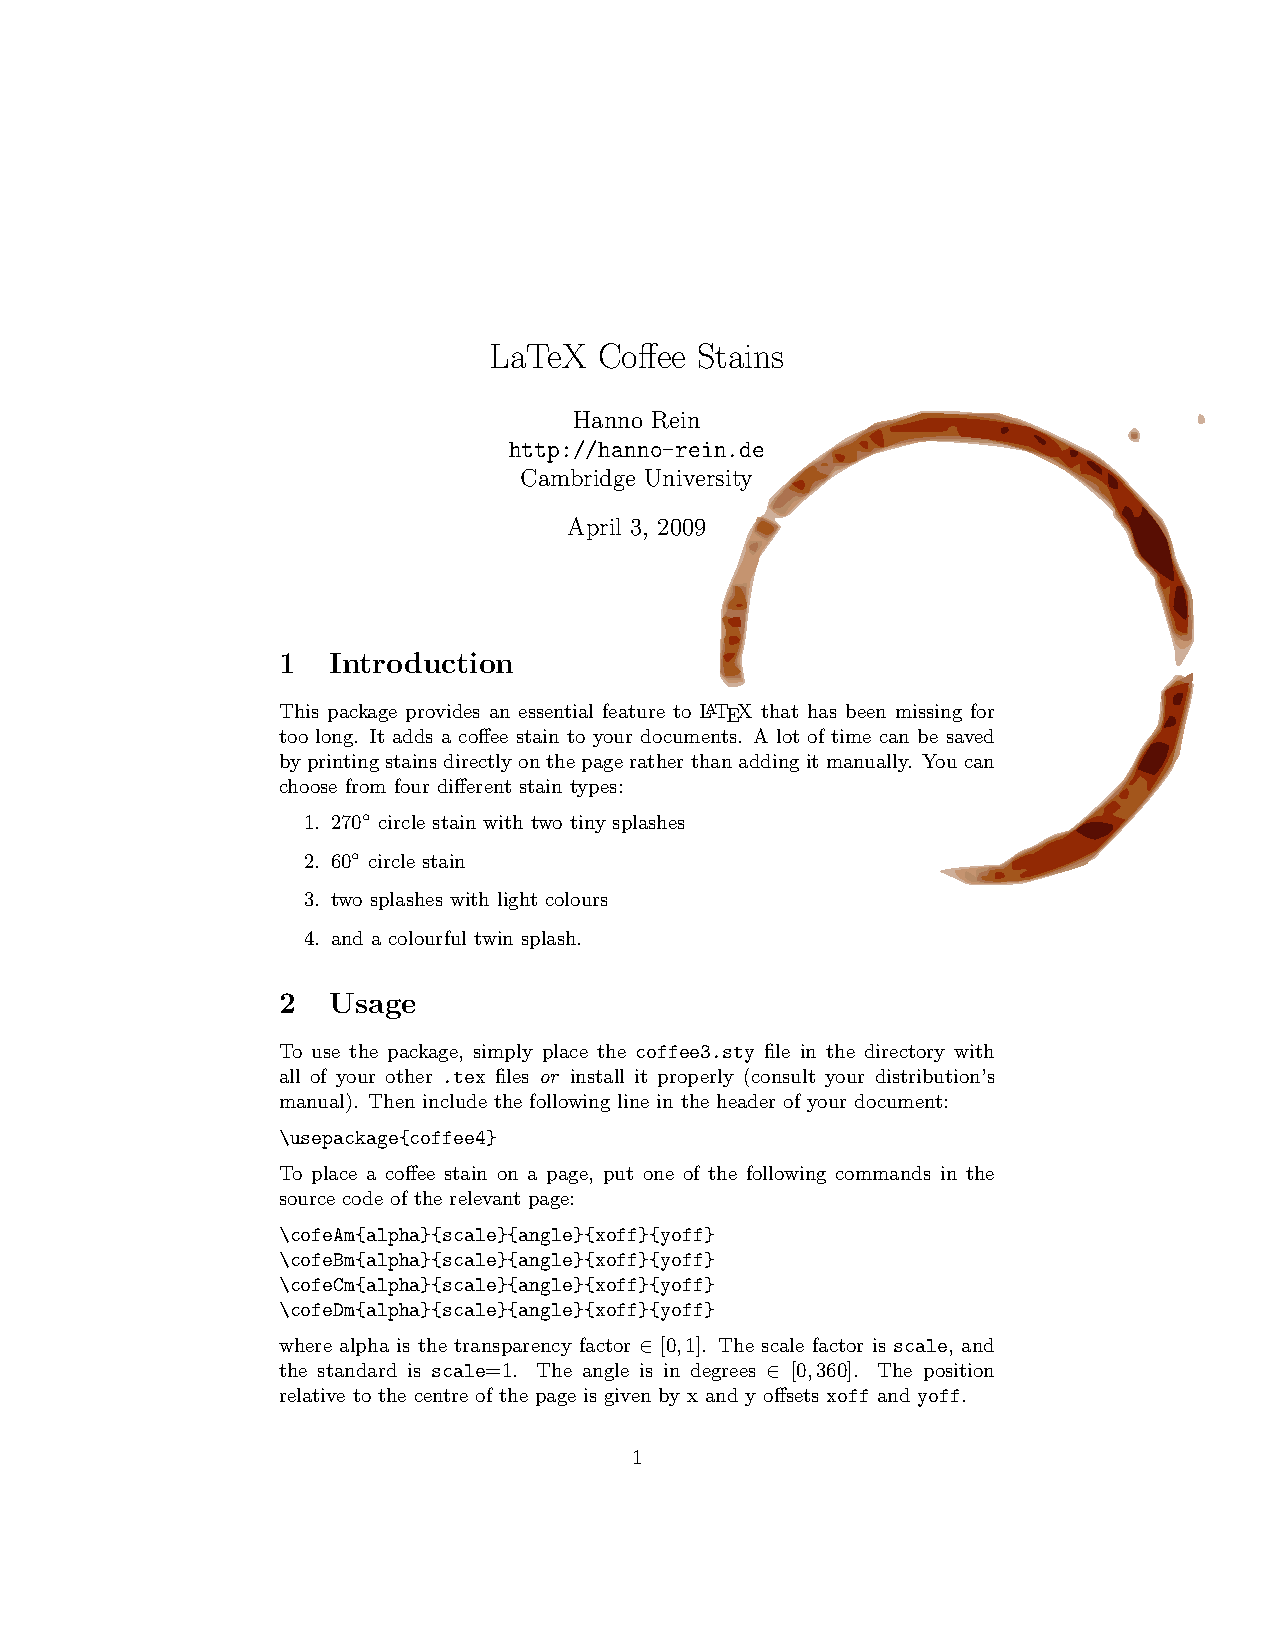
\includegraphics[page=1,width=\textwidth]{coffee4.pdf}
		\end{column}
	\end{columns}
\end{frame}



\begin{frame}{witzige Schriftarten}
	\begin{itemize}[<+->]
		\item \pkg{comicsans}\hfill{\fontspec[Scale=.9]{Comic Sans MS} ziemlich furchtbare Schrift}
		\item \pkg{comicneue}\hfill{\comicneue neuere, nicht ganz so furchtbare Schrift}
                \item \pkg{yfonts}: Gotisch\hfill{\textgoth{eine deutsche Schrift}}
                \item \pkg{yfonts}: Schwabacher\hfill{\textswab{eine sehr deutsche Schrift}}
                \item \pkg{yfonts}: Fraktur\hfill{\textfrak{eine weitere deutsche Schrift}}
%		\item \pkg{ransom}%\hfill{\ransom kaputte Schreibmaschine}
		\item \pkg{cirth}\hfill{\cirth baliN SelN ov fuxiN, lon-d ov monia}
%		\vspace{.2ex}
		\item \pkg{skull}\hfill{|$\textbackslash skull$| \quad \Large \(\skull\)}
                \item \pkg{recycle}\hfill{|\textbackslash recycle| \quad \small \recycle}
		\item \pkg{countriesofeurope}\hfill{\Large\EUCountry{Germany}\EUCountry{Austria}\EUCountry{Italy}\EUCountry{Romania}\EUCountry{Greece}}
		\vspace{-.8em}

		\item \pkg{dancers}\hfill\scalebox{.6}{\dancers Sher­lock Holmes}\hspace{-2ex}\,
	\end{itemize}
\end{frame}

%\begin{frame}{simpsons}
%Schriftart \pkg{simpsons} bietet Simpsons-Charaktere:\\[-.5em]
%|\textbackslash Homer| \uncover<2->{|\textbackslash Left\textbackslash Bart|}\hfill\Homer\uncover<2->{\Left\Bart} \\[2em]\pause\pause
%Position der Pupille anpassbar:\\[-.5em]
%|\textbackslash Goofy\textbackslash Lisa(1,1.6)(.85,1.6)|\hfill\Goofy\Lisa(1,1.6)(.85,1.6) \\[2em]
%\pause
%\hfill \Goofy\Marge(-.5,-.7)(1.5,.8) \Goofy\Maggie(1,-.6)(-.5,-.3) \quad \Left\Burns\hfill\,
%\end{frame}

\begin{frame}[t]{chickenize}
\vfill
	Paket \pkg{chickenize} nutzt Lua um einzelne Buchstaben im \hologo{LuaTeX}-Input zu manipulieren.
	
	\begin{itemize}
		\item Zufälliges wechseln der Schriftart
		\item Färben einzelner Buchstaben
		\item Färben des ganzen Texts als Regenbogen
		\item Ersetzten aller Wörter durch das Wort „Chicken“
		\item Ersetzten aller Buchstaben durch zufällige Buchstaben
		\item …
	\end{itemize}
\end{frame}

\begin{frame}{Edu \LaTeX}
    Es gibt ein Paket eines Heidelbergers, welches vor allem für Aufgabenstellung und Dokumentation für Lehrämtler in der Schule gilt. Ebenfalls gibt es ein ausgegliedertes Paket für Mathematik.

\vspace{1em}
    Einfaches Erstellen von:
    \begin{itemize}
        \item Kapitel, in denen man (Schul-)Mathematik erklärt.
        \item Klausuren in allen Fächern
        \item Zettel als Aufgabenstellung oder auch zur Abgabe
        \item alles andere, was man auch didaktischen Gründen haben möchte…
    \end{itemize}
\vspace{1em}
    Zu finden auf GitHub unter \url{https://github.com/wunderlich/edu} und \url{https://github.com/wunderlich/edumath}
\end{frame}

\begin{frame}{Spaßige Anforderungen}
	Auf \url{tex.stackexchange.com} gibt es immer wieder witzige Fragen …
	\begin{itemize}
		\item \href{http://tex.stackexchange.com/questions/115471/using-contexts-cow-font-with-pdftex}{Using ConTeXts cow font with pdfTeX}
		\item \href{http://tex.stackexchange.com/questions/145223/how-to-draw-a-coffee-cup}{How to draw a coffee cup?}
		\item \href{http://tex.stackexchange.com/questions/63732/cute-child-friendly-document-in-latex}{Cute (child-friendly) document in LaTeX}
		\item \href{http://tex.stackexchange.com/questions/29402/how-do-i-make-my-document-look-like-it-was-written-by-a-cthulhu-worshipping-madm}{How do I make my document look like it was written by a Cthulhu-worshipping madman?}
		\item \href{http://tex.stackexchange.com/questions/74878/create-xkcd-style-diagram-in-tex}{Create xkcd style diagram in TeX}
\item \href{https://tex.stackexchange.com/questions/122116/how-to-prolong-compilation-time-while-engaging-in-leisure-activities}{How to prolong compilation time while engaging in leisure activities?}
	\item \href{https://tex.stackexchange.com/questions/95783/typesetting-the-entire-song-that-never-ends}{Typesetting the entire Song That Never Ends}
	\end{itemize}
\end{frame}

\end{document}
